% !TeX root = ../bbchallenge-paper.tex

\newpage
\subsection{Loops}\label{sec:loops}

\begin{figure}[h!]
  \centering
  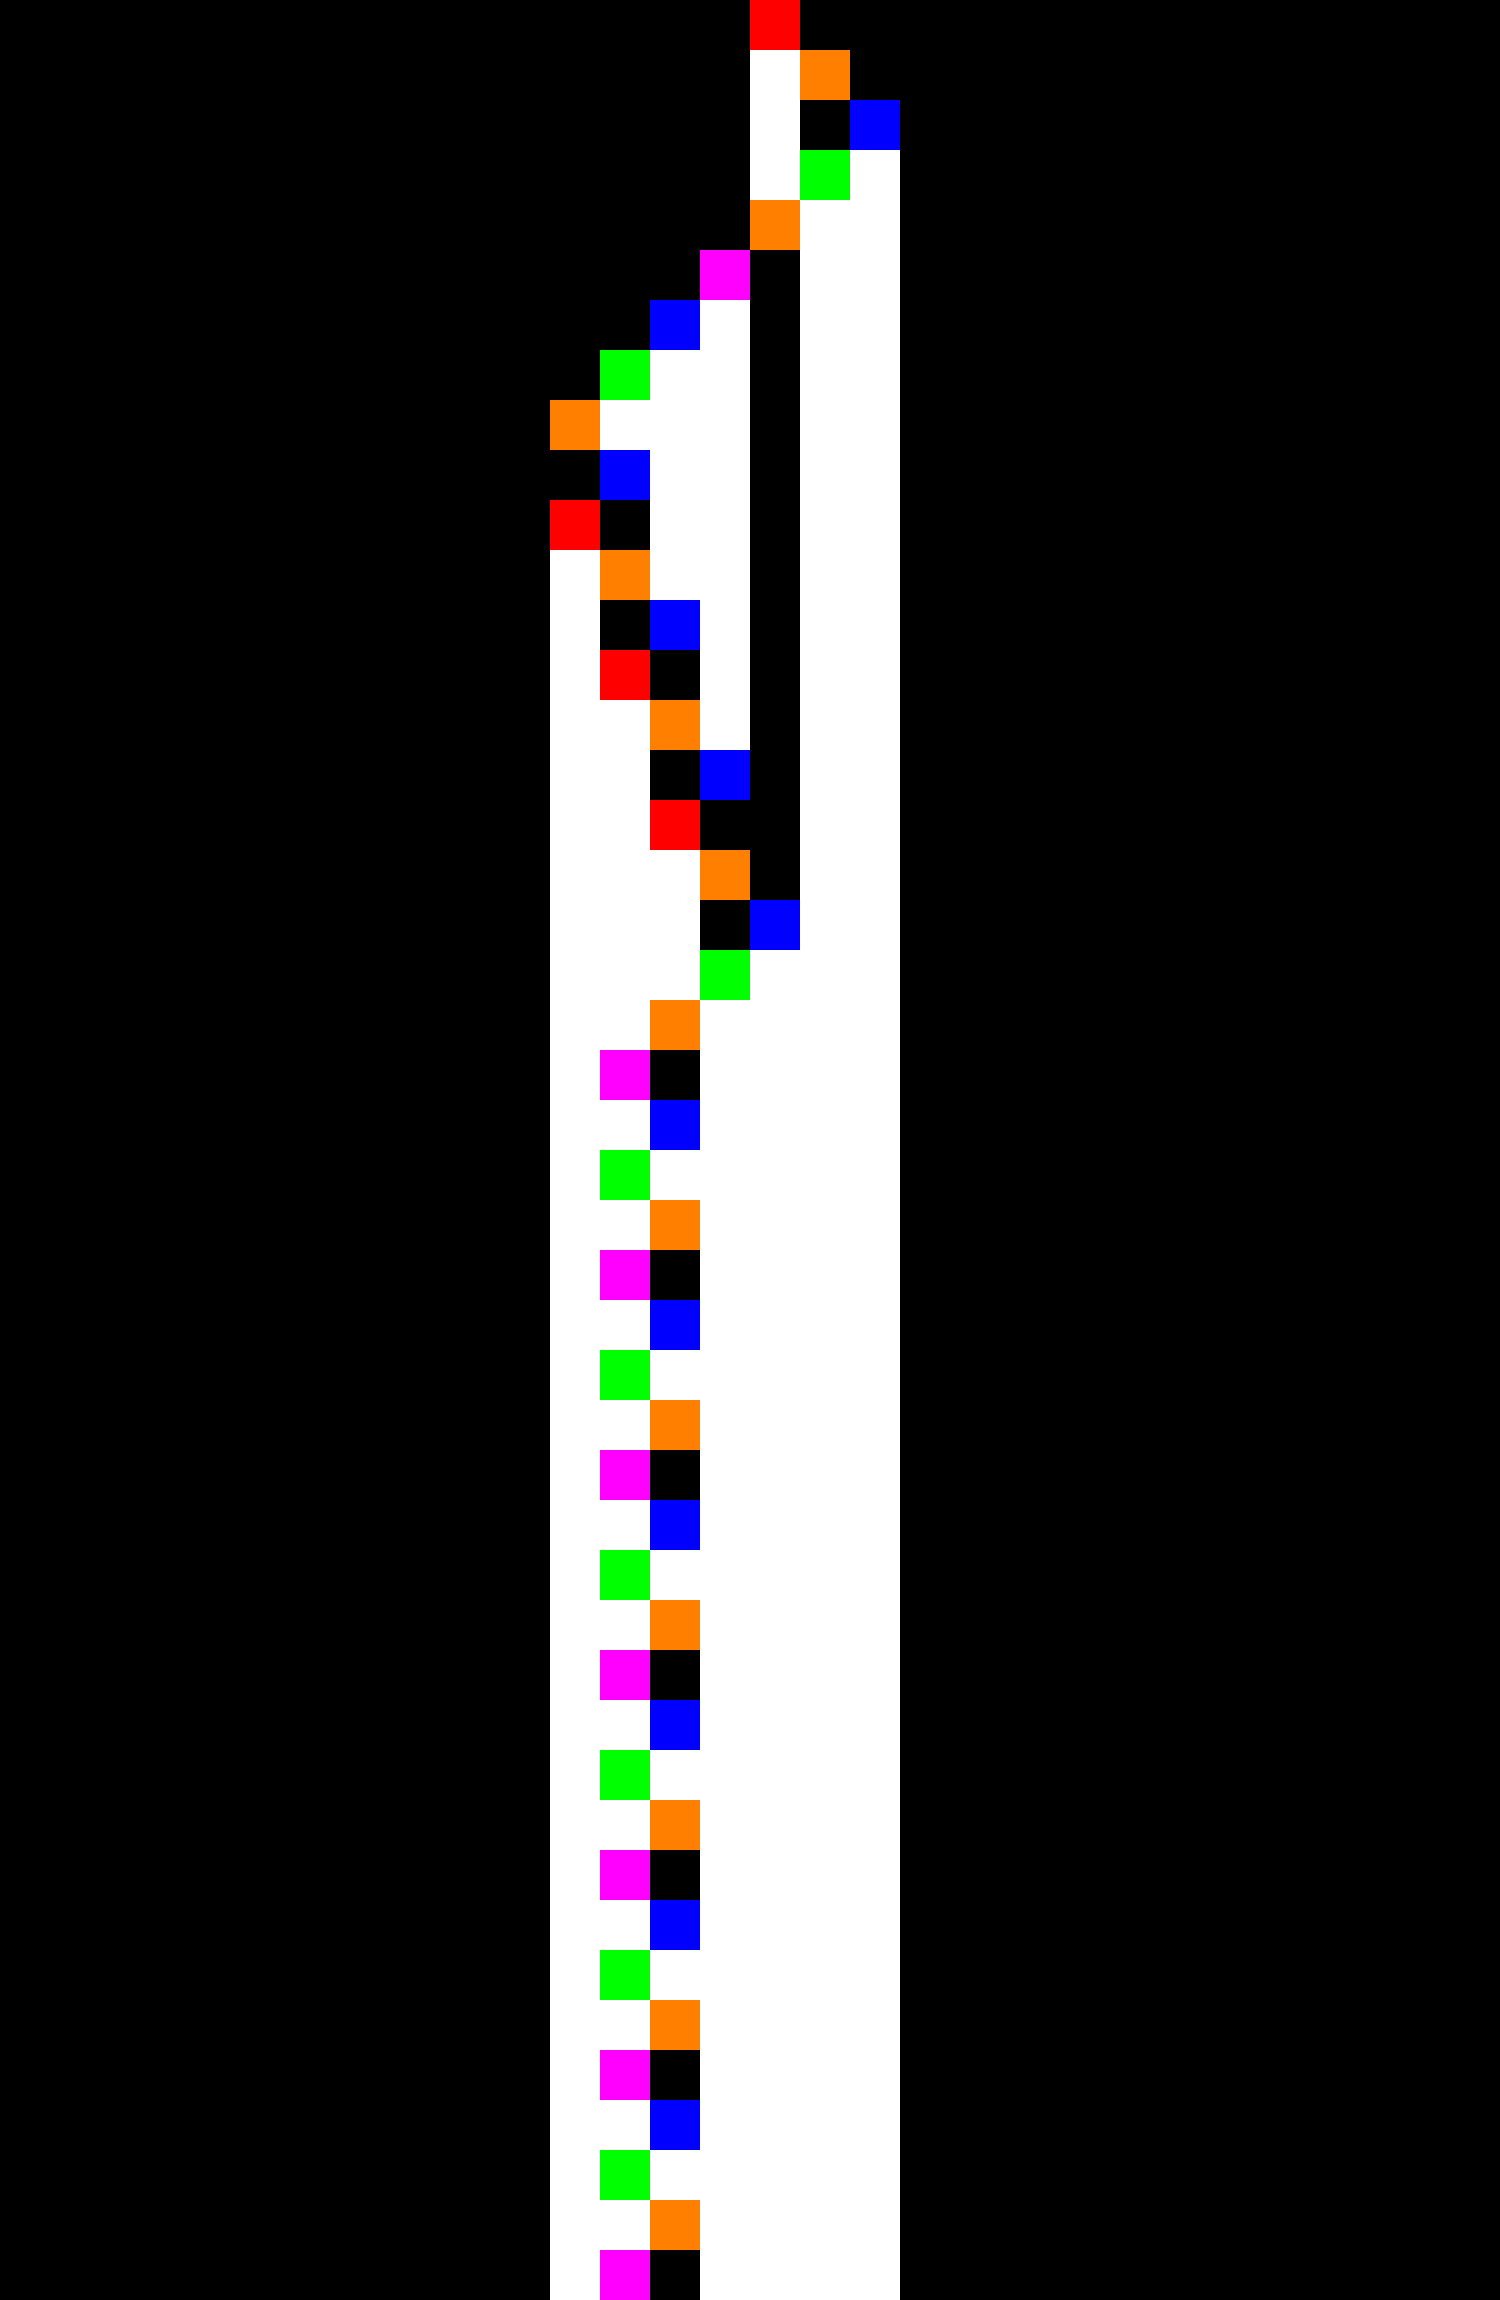
\includegraphics[width=0.4\textwidth]{figures/space-time-diagrams/cycler_279081.pdf}
  \hspace{2ex}
  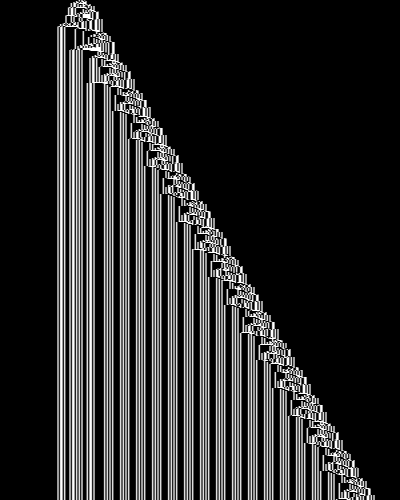
\includegraphics[width=0.4\textwidth]{figures/space-time-diagrams/translated_cycler_59090563_2.png}
  \caption{Space-time diagrams of the 30 first steps of a \textit{\cycler} with colors indicating head position and state (left) and of the 10,000 first steps of a \TC (right). \cyclers are machines that eventually repeat the same configuration forever. \TCs are machines that eventually repeats the same configuration forever, but translated in space. We refer to these two types of machines as \textit{loops}.}\label{fig:loops}
\end{figure}

The goal of this decider is to recognise \textit{Loops} which are Turing machines that eventually repeat the same configuration forever (called \textit{\cyclers}, Figure~\ref{fig:loops}~left), potentially translated in space (called \textit{\TCs}, Figure~\ref{fig:loops}~right).

Deciding Cyclers reduces to the well-known mathematical problem of detecting the cycles of a function for which standard algorithms exist \cite{wiki:Cycle_detection}, the simplest one consisting in memorizing each successive configuration of the machine until encountering one that has been already seen. Translated Cyclers, also known as \textit{Lin's recurrence}, have first been described and decided in Shen Lin's 1963 PhD thesis \cite{Lin1963}, other algorithms to detect them have been developed since then\footnote{\url{https://discuss.bbchallenge.org/t/decider-translated-cyclers/34}}.

Here, we develop a new algorithm (Algorithm~\ref{alg:loops}) for deciding both \cyclers and \TCs. The particularity of this algorithm is that it detects cyclers only by analysing the history of \ssps seen by the machine's head instead of considering entire configurations (\ie with full tape content information). This algorithm is also able to detect if a machine halts and in practice detects 99.99\% of all enumerated halting machines \ts{TS: link to section/table about stats or something and maybe link to the pipeline figure}.

\newpage
\begin{algorithm}
  \caption{{\sc decider-Loops}}\label{alg:loops}

  \begin{algorithmic}[1]
    \State{\textbf{Input:} A Turing machine `$\mathcal{M}$', a step limit parameter $L$.}
    \State{\textbf{Output:} `NON-HALT' if the decider detects that the machine is a loop, `HALT' if the machine halts and `UNKNOWN' otherwise.}

    \State
    \State Simulate $\mathcal{M}$ for $L$ steps and save the history of
    each consecutive state, read-symbol and tape position reached, \ie consecutive $h_i = (s_i,m_i,d_i) \in \states \times \alphabet \times \Z$ for $0 \leq i \leq L$ and $h_0 = (\stateA,\symbolzero,0)$.


    \State \If{the machine has halted before $L$ steps}
    \State \Return HALT
    \EndIf
    \State \For{$l$ \textbf{in} $[0,+\infty[$ } \Comment{$l+1$ is the length of the potential loop}
    \State \If{$2(l + 1) > L$} \Comment{The history does not contain two potential loops of size $l+1$}
    \State \Return UNKNOWN
    \State \EndIf
    \State $K = L-l-1$
    \State $\text{allseen} = \text{true}$
    \State $\text{recordbreak} = \text{false}$
    \State \For{$i$ \textbf{in} $[0,l]$ } \Comment{Comparing \ssp equality at each step of both potential loops}
    \State $s,m,d = h_{L-i}$
    \State $s',m',d' = h_{K-i}$ \Comment{$d'$ will not be used}
    \State \If{$s\neq s'$ \textbf{or} $m \neq m'$}
    \State $\text{allseen} = \text{false}$
    \State \textbf{break}
    \EndIf
    \State \If{$d > \text{max} \{d_j \, | \, j < L-i \}$ \textbf{or} $d < \text{min} \{d_j \, | \, j < L-i \}$}
    \State $\text{recordbreak} = \text{true}$
    \EndIf
    \EndFor
    \State \If{$\text{allseen}$ \textbf{and} ($d_L == d_K$ \textbf{or} $\text{recordbreak}$)}
    \State \Return NON-HALT
    \EndIf
    \EndFor


  \end{algorithmic}
\end{algorithm}